\documentclass[12pt,a4paper,twoside,spanish]{article}      % Libro a 11 pt
\usepackage[utf8]{inputenc}
\usepackage[height=17.5cm,width=13.5cm]{geometry}
\usepackage[spanish]{babel}         % diccionario
\usepackage{epsfig}         % Graficos Postscript
\usepackage{tabularx}
\usepackage{sectsty}
\usepackage{float}
\usepackage{xcolor}
\graphicspath{ {./images/} }
\usepackage{tikz}

\usetikzlibrary{shapes,arrows,positioning}
\tikzstyle{block} = [draw, rectangle, minimum height=3em, minimum width=3em]



%%%%%%%%%%%%%%%%%%%%%%%%%%%%%%%%%%%%%%%%%%%%%%%
%%%%%%%%%%%%%
%%%%%%%%%%%%% Margenes
%%%%%%%%%%%%%
%%%%%%%%%%%%%%%%%%%%%%%%%%%%%%%%%%%%%%%%%%%%%%%
%%%%% Definimos el maximo tamaño posible.
\marginparwidth 0pt     \marginparsep 0pt
\topmargin   0pt        \textwidth   6.5in
\textheight 23cm

% Margen izq del txt en impares.
\setlength{\oddsidemargin}{.0001\textwidth}

% Margen izq del txt en pares.
\setlength{\evensidemargin}{-.04\textwidth}

% Anchura del texto
\setlength{\textwidth}{.99\textwidth}


%%%%%%%%%%%%%%%%%%%%%%%%%%%%%%%%%%%%%%%%%%%%%%%
%%%%%%%%%%%%%
%%%%%%%%%%%%% Profundidad de enumeracion y tabla de contenidos
%%%%%%%%%%%%%
%%%%%%%%%%%%%%%%%%%%%%%%%%%%%%%%%%%%%%%%%%%%%%%

\setcounter{secnumdepth}{3}
\setcounter{tocdepth}{3}


%%%%%%%%%%%%%%%%%%%%%%%%%%%%%%%%%%%%%%%%%%%%%%%
%%%%%%%%%%%%%
%%%%%%%%%%%%% Nuevos Comandos
%%%%%%%%%%%%%
%%%%%%%%%%%%%%%%%%%%%%%%%%%%%%%%%%%%%%%%%%%%%%%

            %%%%%%%%%%%%%%%%%%%%%%%
            %%%%%%%%%%%%%%%%%%%%%%%
            % Comandos para simplificar
            % la escritura
            %%%%%%%%%%%%%%%%%%%%%%%
            %%%%%%%%%%%%%%%%%%%%%%%

\def\mc{\multicolumn}
            %%%%%%%%%%%%%%%%%%%%%%%
            % Comandos para poder utilizar raggedright en tablas
            %%%%%%%%%%%%%%%%%%%%%%%
\newcommand{\PreserveBackslash}[1]{\let\temp=\\#1\let\\=\temp}
\let\PBS=\PreserveBackslash




%%%%%%%%%%%%%%%%%%%%%%%%%%%%%%%%%%%%%%%%%%%%%%%
%%%%%%%%%%%%%
%%%%%%%%%%%%% Cuerpo del documento
%%%%%%%%%%%%%
%%%%%%%%%%%%%%%%%%%%%%%%%%%%%%%%%%%%%%%%%%%%%%%


\begin{document}

\def\chaptername{Capítulo}
\def\tablename{Tabla}
\def\listtablename{Índice de Tablas}
\chapterfont{\LARGE\raggedleft}

%%%%%%%%%%%%%%%%%%%%%%%%%%%%%%%%%%%%%%%%%%%%%%%%%%%%%%%%%%%%%%%
%%%%%%%%%%%%%%%%%%%%%%%%%%%%%%%%%%%%%%%%%%%%%%%%%%%%%%%%%%%%%%%
% DISEÑO DE LA PAGINA DEL TITULO
%%%%%%%%%%%%%%%%%%%%%%%%%%%%%%%%%%%%%%%%%%%%%%%%%%%%%%%%%%%%%%%
%%%%%%%%%%%%%%%%%%%%%%%%%%%%%%%%%%%%%%%%%%%%%%%%%%%%%%%%%%%%%%%
\pagestyle{empty}

\begin{titlepage}
\setlength{\parindent}{0cm} \setlength{\parskip}{0cm}
\newcommand{\HRule}{\rule{\linewidth}{1mm}}

\vspace*{2cm}
\HRule \\[0.5cm]
\begin{center}
% Letra lineal y negrita
\textsf{\textbf{\large UN SISTEMA BASADO EN CONOCIMIENTO PARA EL DISEÑO ÓPTIMO DE UN COCHE DE F1\\[1.5cm]
Análisis de viabilidad e impacto. \\[0.25cm] Modelado del Contexto en CommonKADS \\[0.5cm]}}
\HRule \vspace*{4cm}

\textsf{\textbf{\normalsize Yago Fernández Rego\\Rodrigo Naranjo González\\Adrián Rodríguez López\\[1cm]
Grupo de prácticas: 3.1\\[3.5cm]}}

\textsf{\textbf{\small Desarrollo de Sistemas Inteligentes\\
Universidade da Coruña \\ Curso 2023}}
\end{center}
\end{titlepage}

\cleardoublepage

%%%%%%%%%%%%%%%%%%%%%%%%%%%%%%%%%%%%%%%%%%%%%%%
%%
%% TABLA DE CONTENIDOS
%%
%%%%%%%%%%%%%%%%%%%%%%%%%%%%%%%%%%%%%%%%%%%%%%%

\pagenumbering{Roman}
\tableofcontents
\cleardoublepage


%%%%%%%%%%%%%%%%%%%%%%%%%%%%%%%%%%%%%%%%%%%%%%%%%%%%%%%%%%%%%%%
%%%%%%%%%%%%%%%%%%%%%%%%%%%%%%%%%%%%%%%%%%%%%%%%%%%%%%%%%%%%%%%
%CONTENIDO DEL DOCUMENTO
%%%%%%%%%%%%%%%%%%%%%%%%%%%%%%%%%%%%%%%%%%%%%%%%%%%%%%%%%%%%%%%
%%%%%%%%%%%%%%%%%%%%%%%%%%%%%%%%%%%%%%%%%%%%%%%%%%%%%%%%%%%%%%%

%numeros arábigos
\pagenumbering{arabic} 
%cabeceras
\pagestyle{myheadings} \markboth{SBC para el diseño óptimo de un coche de F1} {Modelado Contextual en CommonKADS.}

%indentaciones y espaciado entre párrafos
\setlength{\parindent}{1,5cm} \setlength{\parskip}{0,7cm}

%%%%%%%%%%%%%%%%%%%%%%%%%%%%%%%%%%%%%%%%%%%%%%%%%%%%%%%%%%%%%%%%%%%%%%%%%%%%%%%
\section{Análisis de Viabilidad: Modelado de la Organización.}
%%%%%%%%%%%%%%%%%%%%%%%%%%%%%%%%%%%%%%%%%%%%%%%%%%%%%%%%%%%%%%%%%%%%%%%%%%%%%%%



%%%%%%%%%%%%%%%%%%%%%%%%%%%%%%%%%%%%%%%%%%%%%%%%%%%%%%%%%%%%%%%%%%%%%%%%%%%%%%%
\subsection{Formulario OM-1: contexto organizacional, problemas y soluciones.}
%%%%%%%%%%%%%%%%%%%%%%%%%%%%%%%%%%%%%%%%%%%%%%%%%%%%%%%%%%%%%%%%%%%%%%%%%%%%%%%


\begin{table}[H]
\scriptsize
\begin{tabularx}{\textwidth}{|l|X|} \hline
\textbf{Modelo de Organización} & \textbf{Formulario OM-1: Problemas y Posibilidades de Mejora} \\ \hline\hline

\textsc{Problemas y Oportunidades} & El principal objetivo de las escuderías en la Fórmula 1 es ganar carreras y campeonatos mundiales, para aumentar así su visibilidad y conseguir la mayor cantidad de beneficios posible, tanto por incentivos gracias a las posiciones en el campeonato como por pagos de patrocinadores. En este caso, los ingenieros deben manejar una gran cantidad de datos para guiar a los mecánicos a realizar las modificaciones necesarias en cada monoplaza. Esto requiere de mucho tiempo, y no son capaces de adaptarse correctamente a los cambios, lo que influye negativamente en sus resultados en la competición. Con un SBC se podría acelerar este proceso, mejorando la configuración y el rendimiento de los vehículos. También puede ayudar a reducir costos y a apreciar características no antes vistas, además de reducir la diferencia de las capacidades con respecto a otras escuderías de más alto nivel.
 \\ \hline
\textsc{Contexto Organizacional} & 
La escudería a la que va destinada este SBC se encuentra inmersa en un entorno muy competitivo y exigente. La Fórmula 1 es una disciplina en la que el tiempo y los recursos son esenciales para conseguir los objetivos deportivos y económicos propuestos. En este contexto, para constituirse en una escudería española relevante a nivel mundial y poder entrar en competición por los primeros puestos, la escudería debe mostrarse eficiente en la gestión de sus recursos y la toma de decisiones estratégicas, mientras trabaja en un entorno altamente tecnológico y en constante evolución. De esta forma, se enfrenta a la necesidad de optimizar la configuración de sus coches para cada piloto, según sus preferencias personales y estilo de conducción, y cada circuito, en función del trazado y las características de la pista donde se celebre el Gran Premio. Todo ello para lograr el máximo rendimiento y el mejor resultado en cada carrera. Esto conlleva una gran cantidad de análisis de datos y ajustes técnicos que deben realizarse en un período de tiempo limitado. La capacidad de la escudería para adaptarse rápidamente a las condiciones cambiantes de la pista y a las necesidades de sus pilotos es crucial para el éxito en la Fórmula 1.     
\begin{enumerate} 
        \item Misión: escudería española que forma parte del campeonato mundial de Fórmula 1.
        \item Visión: escudería española altamente reconocida en todo el mundo compitiendo entre los primeros puestos del mundial de Fórmula 1.
        \item Objetivos: conseguir ventaja con respecto a los otros equipos, y conseguir situarse en los primeros puestos de la clasificación durante varios años. 
\end{enumerate}\\ \hline
\textsc{Soluciones} & La solución que se propone es el desarrollo de un SBC que 
 nos proporcione la configuración óptima del monoplaza en base a las preferencias personales de cada piloto y las características del circuito. \\
\hline
\end{tabularx}
  \label{tab.OM1}
\end{table}




%%%%%%%%%%%%%%%%%%%%%%%%%%%%%%%%%%%%%%%%%%%%%%%%%%%%%%%%%%%%%%%%%%%%%%%%%%%%%%%
\pagebreak
\subsection{Formulario OM-2: descripción del área de interés de la organización.}
%%%%%%%%%%%%%%%%%%%%%%%%%%%%%%%%%%%%%%%%%%%%%%%%%%%%%%%%%%%%%%%%%%%%%%%%%%%%%%%

\begin{table}[H]
\scriptsize
\begin{tabularx}{\textwidth}{|l|X|} \hline
\textbf{Modelo de Organización} & \textbf{Formulario OM-2: Aspectos Variables} \\ \hline\hline

\textsc{Estructura} & 
\begin{center}
    
    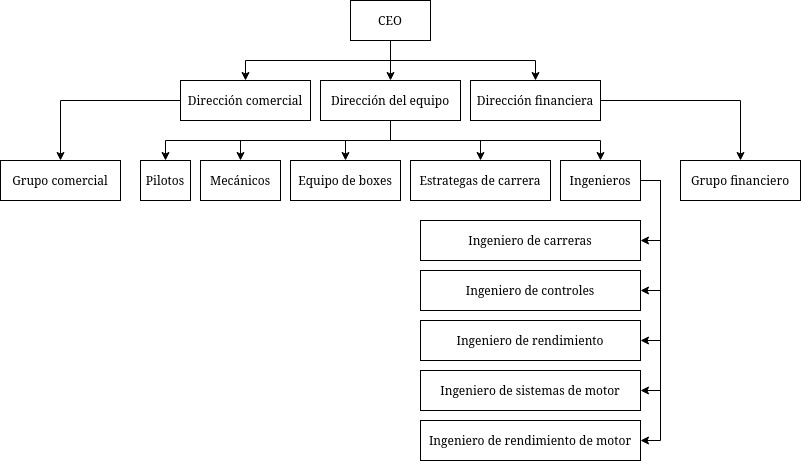
\includegraphics[scale=0.4]{estructura.jpg}
\end{center}
\\ \hline
\textsc{Procesos} & Mediante el análisis de los datos ofrecidos, se ha concluido que el único proceso es:
\begin{itemize}
    \item Optimizar las características técnicas y mecánicas para cada monoplaza según las preferencias de los pilotos y las condiciones de la pista.
\end{itemize} \\ \hline
\textsc{Personal} &  Los mecánicos de la escudería serán los encargados de manejar y alterar las distintas piezas y componentes que se requieran. Además, cada piloto podrá involucrarse para informar sobre sus preferencias y sensaciones en la conducción que puedan resultar de utilidad para los mecánicos al modificar sus respectivos coches. Por último, será el trabajo del equipo de ingenieros de la escudería al completo los que se encarguen de analizar e informar de los datos de la pista, la meteorología, y el asfalto. Todo ello siempre será supervisado por el director del equipo.  \\ \hline
\textsc{Recursos} &  De la información recopilada por medio de sensores y radares (temperatura, presión, viento, previsiones meteorológicas, etc.), o gracias al conocimiento previo de ingenieros y pilotos (aerodinámica, trazado, etc.), se obtendrá una serie de parámetros que se deberán tener en cuenta para la modificación de los componentes con las herramientas y los recursos mecánicos de los que disponga la escudería (motor, alerones, suspensión, etc.).
\\ \hline
\textsc{Conocimiento} &  Véase OM-4. \\ \hline
\textsc{Cultura y Potencial} &  La estrategia del equipo prevalecerá sobre las opiniones del piloto.\\ \hline
\end{tabularx}
  \label{tab.OM2}
\end{table}



%%%%%%%%%%%%%%%%%%%%%%%%%%%%%%%%%%%%%%%%%%%%%%%%%%%%%%%%%%%%%%%%%%%%%%%%%%%%%%%
\pagebreak
\subsection{Formulario OM-3: descomposición del proceso de negocio.}
%%%%%%%%%%%%%%%%%%%%%%%%%%%%%%%%%%%%%%%%%%%%%%%%%%%%%%%%%%%%%%%%%%%%%%%%%%%%%%%

\begin{table}[H]
\scriptsize
\begin{tabularx}{\textwidth}{|p{0.2cm}|>{\raggedright}X|>{\raggedright}X|>{\raggedright}X|>{\raggedright}X|>{\raggedright}X|>{\PBS\raggedright}X|} \hline
\multicolumn{3}{|l}{\textbf{Modelo de Organización}} &
\multicolumn{4}{|l|}{\textbf{Formulario OM-3: Descomposición de
los Procesos}}\\ \hline\hline \textsc{N\textordmasculine} &
\textsc{Tarea} &  \textsc{Realiza\-da por} &  \textsc{¿Dónde?} &
\textsc{Recursos de Conocimiento} & \textsc{¿In\-ten\-si\-va en
Conocimiento?} & \textsc{Im\-por\-tan\-cia} \\ \hline 

1 & 
Recogida de datos de la pista. & 
Equipamiento de sensores. &
Circuito. & 
No. &
No. & 
Requisito necesario para iniciar el proceso. \\ \hline 

2 &
Diagnóstico de los datos en busca de anomalías. & 
Ingenieros. &
\textit{Pit wall} del circuito donde se encuentran los monitores de la escudería. & 
Experiencia y conocimiento de los recursos involucrados. &
Sí. & 
Recomendable. \\ \hline 

3 & 
Recopilación de las preferencias del piloto. & 
Pilotos. &
N/A. & 
Experiencia y conocimiento de los recursos involucrados. &
Sí, pero no requiere razonamiento intensivo.  & 
Opcional. \\ \hline 

4 &
Generación de la configuración óptima del monoplaza. & 
Ingenieros y director del equipo. &
\textit{Pit wall} del circuito donde se encuentran los monitores de la escudería. & 
Conocimiento del reglamento y experiencia en generación de configuraciones. &
Sí, de razonamiento elevado. & 
Paso clave. \\ \hline

5 &
Modificación del monoplaza respecto a la solución propuesta. & 
Mecánicos. &
Garaje de la escudería en los boxes del circuito. & 
Experiencia y conocimiento en mecánica de los recursos involucrados. &
Sí. & 
Requisito necesario. \\ \hline

6 &
Prueba en pista de la configuración realizada. & 
Pilotos. &
Circuito. & 
Experiencia de conducción por parte del piloto y conocimiento del circuito. &
Sí, pero no requiere razonamiento intensivo. & 
Recomendable. \\ \hline

7 &
Evaluación de la solución propuesta y los datos conseguidos por la prueba en pista. & 
Ingenieros y director del equipo. &
\textit{Pit wall} del circuito. & 
Experiencia, conocimiento del reglamento y conocimiento técnico de los recursos involucrados. &
Sí, de razonamiento elevado. & 
Recomendable. \\ \hline

\end{tabularx}
\label{tab.OM3}
\end{table}



%%%%%%%%%%%%%%%%%%%%%%%%%%%%%%%%%%%%%%%%%%%%%%%%%%%%%%%%%%%%%%%%%%%%%%%%%%%%%%%
\pagebreak
\subsection{Formulario OM-4: activos de conocimiento.}
%%%%%%%%%%%%%%%%%%%%%%%%%%%%%%%%%%%%%%%%%%%%%%%%%%%%%%%%%%%%%%%%%%%%%%%%%%%%%%%

\begin{table}[H]
\scriptsize
\begin{tabularx}{\textwidth}{|>{\raggedright}X|>{\raggedright}X|>{\raggedright}X|>{\raggedright}X|>{\raggedright}X|>{\raggedright}X|>{\PBS\raggedright}X|} \hline
\multicolumn{3}{|l}{\textbf{Modelo de Organización}} & \multicolumn{4}{|l|}{\textbf{Formulario OM-4: Activos de Conocimiento}} \\ \hline\hline
\textsc{Recurso de Conocimiento} & \textsc{Pertenece a} &  \textsc{Usado en} &  \textsc{¿Forma
Correcta?} & \textsc{¿Lugar Correcto?} & \textsc{¿Tiempo Correcto?} & \textsc{¿Calidad Correcta?}\\ \hline

Experiencia en generación de configuraciones. & 
Ingenieros y director de equipo. &
Tarea 4 & 
No, reside en los recursos involucrados. & 
Sí. &
No, el tiempo empleado puede resultar excesivo. & 
No, la solución puede no ser óptima porque no puede probar todas las opciones.\\ \hline

Experiencia y conocimiento en mecánica. & 
Mecánicos. &
Tarea 5 & 
No, reside en los recursos involucrados. & 
Sí. &
No, el tiempo empleado puede resultar excesivo. & 
No, puede haber fallos que ocasionen problemas mecánicos en el coche.\\ \hline

Experiencia de conducción y conocimiento del circuito. & 
Pilotos. &
Tarea 6 & 
No, reside en los pilotos. & 
Sí. &
No, el tiempo empleado puede resultar excesivo & 
No, puede llevar a fallos de conducción o accidentes.\\ \hline

Conocimiento e interpretación del reglamento. & 
Ingenieros, director del equipo. &
Tareas 4 y 7 & 
No, reside en los recursos involucrados. & 
Sí. &
No, el tiempo empleado puede resultar excesivo. & 
No, puede incurrir en infracciones y sanciones.\\ \hline

\end{tabularx}
  \label{tab.OM4}
\end{table}

%%%%%%%%%%%%%%%%%%%%%%%%%%%%%%%%%%%%%%%%%%%%%%%%%%%%%%%%%%%%%%%%%%%%%%%%%%%%%%%
\pagebreak
\subsection{Formulario OM-5: Análisis de viabilidad.}
%%%%%%%%%%%%%%%%%%%%%%%%%%%%%%%%%%%%%%%%%%%%%%%%%%%%%%%%%%%%%%%%%%%%%%%%%%%%%%%

\begin{table}[H]
\scriptsize
\begin{tabularx}{\textwidth}{|l|X|} \hline


\textbf{Modelo de Organización} & \textbf{Formulario OM-5: Elementos del Documento de Viabilidad}\\ \hline\hline
\textsc{Viabilidad Empresarial} & 
Configurar un coche de F1 es un trabajo principalmente largo; desde el momento en el que se obtienen los datos, se analizan, se toma la decisión de qué cambiar, hasta que se modifica el coche. Todo ello provoca un coste excesivo en tiempo para la escudería, con resultados que finalmente pueden no ser los adecuados, incompletos o directamente incorrectos. Para estimar el coste del proyecto, analizaremos los costes de cada una de sus fases. Empezaremos con el análisis del contexto, tarea desempeñada por 2 analistas durante 35 días, con un coste de 12.000 €. La segunda fase es el modelado conceptual, desempeñado por dos Ingenieros de Conocimiento con la ayuda de un experto durante un mes, suponiendo un coste de 16.000€. Posteriormente se procederá a diseñar el software con dos desarrolladores durante 40 días, y con un coste de 14.000€. Tras el diseño pasaremos a implementar dicho software, con cuatro desarrolladores durante 20 días, por lo que el coste serán 12.000€. Finalmente, testearemos el trabajo realizado con dos testers durante 15 días, con un costo de 8.000€. 
Dicho esto, podemos concluir que el coste del proyecto serán 62.000€, y aunque no proporcione ningún beneficio económico directo, sí ayudará a ahorrar en gastos derivados por soluciones inadecuadas y a mejorar considerablemente la fiabilidad y gestión de la parte mecánica de la configuración. Además, permitirá ahorrar tiempo en tareas tediosas, pudiendo dedicar esos esfuerzos a otras actividades. Esto llevará a mejores resultados, que harán de la escudería un producto deseable a los patrocinadores, aumentando enormemente el beneficio a largo plazo y la capacidad. Otra ventaja es la carencia de riesgos, pues los datos existentes y las soluciones pueden ser revisadas rápidamente, y los datos nuevos pueden ser añadidos rápidamente para adaptar el sistema a situaciones como cambios repentinos en la meteorología, sustituciones de algún piloto, o la falta de algún componente. Este proyecto se adecúa a cualquier organización del mundo del motor, y no existen, o al menos no están distribuidas libremente, herramientas similares basadas en SBCs. \\ \hline


\textsc{Viabilidad Técnica} & 
Se espera que el SBC sea capaz de alcanzar la configuración óptima en base a los datos proporcionados, y las piezas y capacidades disponibles. El principal aspecto crítico es el tiempo, y se espera obtener la mejor solución en el menor tiempo posible. No se priorizará la sencillez o belleza de la interfaz, pues el sistema se centrará en la funcionalidad. Los ingenieros están habituados a tratar con aplicaciones de apariencia similar y cuentan con los conocimientos necesarios para manejarla. Además, estos no se verán afectados en su trabajo habitual. El éxito del proyecto queda determinado por la obtención de una solución completa y de calidad, y por el grado de aceptación de los recursos involucrados. \\ \hline

\textsc{Viabilidad del Proyecto} & 
De toda la información recogida hasta el momento se puede afirmar que el compromiso del personal es alto, pues el SBC facilitará y mejorará la obtención de resultados por parte de la escudería y aportará una mayor ventaja con respecto al resto de constructores. Se requerirá el conocimiento del experto, el cual estará a nuestra disposición en la medida de lo posible, y el conocimiento técnico del reglamento, ya establecido y consultable en cualquier momento. Aunque el tamaño del conocimiento que se almacene sea medio, la dificultad radicará en la gran cantidad de combinaciones que se puedan dar en base a la diversidad de los datos disponibles, y en la experiencia técnica del equipo de mecánicos para llevar a cabo las soluciones propuestas.  \\ \hline



\textsc{Acciones Propuestas} & 
Nos centraremos en conseguir mejorar el manejo de datos de los ingenieros y la rapidez con la que encuentran las mejores configuraciones para conseguir que los mecánicos trabajen de la forma más eficaz posible y realizando su trabajo con mayor calidad. Para ello, automatizaremos la tarea de generación óptima del monoplaza mediante un SBC (véase Tarea 4 del OM-3). \\ \hline
\end{tabularx}
\caption{Formulario OM-5.}
  \label{tab.OM5_2}
\end{table}


%%%%%%%%%%%%%%%%%%%%%%%%%%%%%%%%%%%%%%%%%%%%%%%%%%%%%%%%%%%%%%%%%%%%%%%%%%%%%%%
\pagebreak
\section{Análisis de Impactos y Mejoras: Modelado de las Tareas y los Agentes.}
%%%%%%%%%%%%%%%%%%%%%%%%%%%%%%%%%%%%%%%%%%%%%%%%%%%%%%%%%%%%%%%%%%%%%%%%%%%%%%%
\subsection{Formulario TM-1: análisis de tareas.}
%%%%%%%%%%%%%%%%%%%%%%%%%%%%%%%%%%%%%%%%%%%%%%%%%%%%%%%%%%%%%%%%%%%%%%%%%%%%%%%

\begin{table}[H]
\scriptsize
\begin{tabularx}{\textwidth}{|l|X|} \hline

\textbf{Modelo de Tareas} & \textbf{Formulario TM-1: Análisis de Tareas} \\ \hline\hline

\textsc{Tarea} & 
Tarea 4. Generación de la configuración óptima del monoplaza\\ \hline

\textsc{Organización}  & 
Es responsabilidad de los ingenieros, supervisados por el director del equipo. \\ \hline

\textsc{Objetivo y valor} & 
Generar una configuración que permita el máximo rendimiento del coche, sin violar las restricciones (véanse más abajo) y cumpliendo el mayor número de preferencias del piloto.\\ \hline

\textsc{Dependencia y Flujos} &
\textit{Tareas precedentes:} imprescindible la recogida de datos que se aportarán al SBC para su correcto funcionamiento (tarea 1), y opcionalmente las tareas 2 y 3. \\ &
\textit{Tareas consecuentes:} una vez obtenida la solución, se deberá, como mínimo indispensable, llevar a cabo la modificación del monoplaza (tarea 5). \\ \hline

\textsc{Objetos manipulados} &
\textit{1. Objetos de entrada:} datos provenientes de los sensores respecto a variables del entorno (temperatura, viento, presión, etc.), preferencias de los pilotos, datos fijos acerca del trazado del circuito (número de curvas, velocidades máximas alcanzadas, tiempo medio de vuelta, etc.). \\ &
\textit{2. Objetos de salida:} especificaciones y cambios que permitan la reproducción de la solución propuesta.\\ &
\textit{3. Objetos internos:} configuraciones generadas por el sistema durante su funcionamiento, reglamento que influirá en las opciones de configuración. \\ \hline

\textsc{Tiempo y control} & 
\textit{1. Frecuencia y duración:} la tarea se ejecuta cada día que el monoplaza sale a la pista (si se desea), una o varias veces, y su duración será variable y dependiente de la complejidad de los datos y el circuito. \\ & 
\textit{2. Restricciones:} la solución propuesta debe poder reproducirse con los recursos y capacidades disponibles en ese momento. \\ \hline

\textsc{Agentes} &
Ingenieros y director de equipo.\\ \hline

\textsc{Conocimiento y Capacidad} &
Es imprescindible el conocimiento del reglamento, así como la capacidad de manejar el conocimiento técnico de esta tarea a un nivel experto, y la experiencia previa en esta actividad. \\ \hline

\textsc{Recursos} &
El recurso principal es el tiempo, ya que obtener una configuración consume mucho tiempo y es una tarea que puede estar sujeta a iteraciones. También se hará uso de software especializado (para cálculos, mediciones, etc.), ya disponible por la propia escudería. \\ \hline

\textsc{Calidad y eficiencia} &
La evaluación de la calidad de la solución se realizará a posteriori (tarea 7), si es posible, y tras realizar las pruebas pertinentes en pista (tarea 6).
\\ \hline

\end{tabularx}

  \label{tab.TM1}
\end{table}

%%%%%%%%%%%%%%%%%%%%%%%%%%%%%%%%%%%%%%%%%%%%%%%%%%%%%%%%%%%%%%%%%%%%%%%%%%%%%%%
\pagebreak
\subsection{Formulario TM-2: análisis de los cuellos de botella del conocimiento.}
%%%%%%%%%%%%%%%%%%%%%%%%%%%%%%%%%%%%%%%%%%%%%%%%%%%%%%%%%%%%%%%%%%%%%%%%%%%%%%%

\begin{table}[H]
\scriptsize
\begin{tabularx}{\textwidth}{|p{5cm}|>{\PBS\raggedright}p{0.8cm}|X|} \hline
\textbf{Modelo de Tareas} & \multicolumn{2}{l|}{\textbf{Formulario TM-2: Elemento de Co\-no\-ci\-mien\-to}} \\ \hline\hline
\textsc{Nombre} &  \multicolumn{2}{p{8cm}|}{Conocimiento y experiencia en generación de configuraciones}\\ \hline
\textsc{Poseído por} &  \multicolumn{2}{X|}{Ingenieros y director de equipo}\\ \hline
\textsc{Usado en} &  \multicolumn{2}{l|}{Tarea 4}\\ \hline
\textsc{Dominio} &  \multicolumn{2}{p{7.5cm}|}{Ingeniería mecánica, especializada en monoplazas de altas prestaciones.}\\ \hline

\textbf{Naturaleza del conocimiento} & \emph{(Sí/No)} &
\textbf{¿Supone un cuello de botella?¿Debe ser mejorado?}\\ 
\hline Formal, riguroso & & \\ 
\hline Empírico, cuantitativo& & \\
\hline Heurístico, sentido común& X & \\
\hline Altamente especializado, específico del dominio& X & \\
\hline Basado en la experiencia& X & \\
\hline Basado en la acción$^1$& & \\
\hline Incompleto& X & Si, pero no puede mejorarse con el SBC\\
\hline Incierto, puede ser incorrecto & X& Mejorable en el SBC\\
\hline Cambia con rapidez& &\\
\hline Difícil de verificar& & \\
\hline Tácito, difícil de transferir& X & Mejorable en el SBC\\
\hline \textbf{Forma del conocimiento} & &\\ 
\hline Mental& X & Explicitado en el SBC \\
\hline Papel& & \\
\hline Electrónica& & \\
\hline Habilidades& X & \\
\hline Otros& & \\
\hline \textbf{Disponibilidad del Conocimiento} &  &\\
\hline Limitaciones en tiempo& X & Sí, paliable con el SBC\\ 
\hline Limitaciones en espacio& & \\ 
\hline Limitaciones de acceso& &  \\
\hline Limitaciones de calidad& X & Si, paliable con el SBC \\
\hline Limitaciones de forma& & \\
\hline
\end{tabularx}
  \label{tab.TM2}
\end{table}

\pagebreak

\begin{table}[H]
\scriptsize
\begin{tabularx}{\textwidth}{|p{5cm}|>{\PBS\raggedright}p{0.8cm}|X|} \hline
\textbf{Modelo de Tareas} & \multicolumn{2}{l|}{\textbf{Formulario TM-2: Elemento de Co\-no\-ci\-mien\-to}} \\ \hline\hline
\textsc{Nombre} & \multicolumn{2}{p{7.5cm}|}{Interpretación del reglamento}\\ \hline
\textsc{Poseído por} & \multicolumn{2}{X|}{Ingenieros y director de equipo}\\ \hline
\textsc{Usado en} & \multicolumn{2}{l|}{Tarea 4}\\ \hline
\textsc{Dominio} & \multicolumn{2}{p{7.5cm}|}{Reglamentación y estándares de seguridad a nivel legislativo, especializado en mecánica.}\\ \hline

\textbf{Naturaleza del conocimiento} & \emph{(Sí/No)} & \textbf{¿Supone un cuello de botella?¿Debe ser mejorado?}\\ 
\hline Formal, riguroso & & \\\hline Empírico, cuantitativo& & \\ \hline
Heurístico, sentido común& X & \\ \hline Altamente especializado,
específico del dominio& X & \\ \hline Basado en la experiencia& X & \\
\hline Basado en la acción$^1$& & \\ \hline Incompleto& X & Si, pero no puede mejorarse con el SBC\\
\hline Incierto, puede ser incorrecto & X& Mejorable con el SBC.\\ \hline Cambia con
rapidez& X&
\\ \hline Difícil de verificar& & \\ \hline Tácito, difícil de
transferir& X & Mejorable con el SBC\\ \hline \textbf{Forma del conocimiento} &  &\\ \hline
Mental& X & Explicitado en el SBC\\ \hline Papel& & \\ \hline Electrónica& & \\ \hline
Habilidades& & \\ \hline Otros& & \\ \hline \textbf{Disponibilidad
del Conocimiento} &  &\\ \hline Limitaciones en tiempo& X & Si, Paliable con el SBC \\ \hline
Limitaciones en espacio& & \\ \hline Limitaciones de acceso & & \\
\hline Limitaciones de calidad & X & Si, paliable con el SBC. \\ \hline Limitaciones de forma& &
\\ \hline
\end{tabularx}
  \label{tab.TM2}
\end{table}

{\scriptsize \noindent $^1$ Se refiere a conocimiento que se
adquiere con la repetición de actividades físicas tales como
conducir, encestar, etc.}

%%%%%%%%%%%%%%%%%%%%%%%%%%%%%%%%%%%%%%%%%%%%%%%%%%%%%%%%%%%%%%%%%%%%%%%%%%%%%%%
\pagebreak
\subsection{Formulario AM-1: descripción de los agentes.}
%%%%%%%%%%%%%%%%%%%%%%%%%%%%%%%%%%%%%%%%%%%%%%%%%%%%%%%%%%%%%%%%%%%%%%%%%%%%%%%

\begin{table}[H]
\scriptsize
\begin{tabularx}{\textwidth}{|l|X|} \hline
\textbf{Modelo de Agentes} & \textbf{Formulario AM-1: Agentes} \\ \hline\hline
\textsc{Nombre} &  
Director del equipo.
\\ \hline

\textsc{Organización} &  
Tal como se puede ver en el organigrama presentado en el OM-2, el director del equipo responde directamente ante el CEO de la escudería, y se encarga de representarla de cara al público. Su trabajo es controlar al equipo en pista y tomar las decisiones del día a día de la escudería.
\\ \hline

\textsc{Implicado en} & 
Está implicado las tareas 4 y 5.
\\ \hline

\textsc{Se comunica con} & 
El equipo de ingenieros y los pilotos.
\\ \hline

\textsc{Conocimiento} &  
Su conocimiento y experiencia, tanto del proceso como del reglamento necesario para llevarlo a cabo, es muy elevado.
\\ \hline

\textsc{Responsabilidades y restricciones} & 
Es el que debe tomar la decisión final sobre la configuración que se decidirá llevar a cabo en el monoplaza, así como supervisar el proceso para asegurarse de que los ingenieros estén realizando su trabajo de forma correcta.
\\ \hline
\end{tabularx}
 \label{tab.AM1}
\end{table}

\begin{table}[H]
\scriptsize
\begin{tabularx}{\textwidth}{|l|X|} \hline
\textbf{Modelo de Agentes} & \textbf{Formulario AM-1: Agentes} \\ \hline\hline
\textsc{Nombre} &  
Ingenieros.
\\ \hline

\textsc{Organización} &  
Tal como se puede ver en el organigrama presentado en el OM-2, los ingenieros responden ante el director del equipo. Se dividen en cinco roles, cada uno con sus especialidades, y se disponen, como mínimo, de dos ingenieros de cada especialidad, asignados cada uno a uno de los coches.
\\ \hline

\textsc{Implicado en} & 
Están implicados las tareas 1, 2, 3, 4, y 7.
\\ \hline

\textsc{Se comunica con} & 
El director del equipo, los mecánicos, y los pilotos.
\\ \hline

\textsc{Conocimiento} &  
Son expertos en su campo y disponen de mucha experiencia. Deben conocer bien el reglamento para no incurrir en ilegalidades y aprovechar las zonas grises que permiten configuraciones más arriesgadas.
\\ \hline

\textsc{Responsabilidades y restricciones} & 
Deben generar la configuración con los datos recopilados anteriormente de forma que sea lo más óptima posible, y serán los que harán uso del SBC. Deben esperar a que el director del equipo apruebe su diseño, y deben ceñirse a las restricciones marcadas por el reglamento del organismo regulador de la competición.
\\ \hline
\end{tabularx}
 \label{tab.AM1}
\end{table}

%%%%%%%%%%%%%%%%%%%%%%%%%%%%%%%%%%%%%%%%%%%%%%%%%%%%%%%%%%%%%%%
%FINAL DEL LIBRO
%%%%%%%%%%%%%%%%%%%%%%%%%%%%%%%%%%%%%%%%%%%%%%%%%%%%%%%%%%%%%%%
\end{document}
